\documentclass{llncs}
\usepackage{enumerate,graphicx}
\usepackage{graphicx}
\usepackage{amsmath,amssymb}
\usepackage{algorithm,lipsum}
\usepackage[noend]{algpseudocode}
\usepackage{graphicx}
%\usepackage{titling}

%\newcommand{\subtitle1}[1]{%
%	\posttitle{%
%	\begin{center}\large#1\end{center}
%	\vskip0.5em}%
%}

\title{Safety Critical Systems Project Report \\ Predictive Maintenance in Vehicle Systems}
\author{Pushpita Sarkar(Matriculation No: 1384152)\and Nidhi Nayak (Matriculation No: 1404524)\and Deepak Kumar (Matriculation No: 1400489)\and Ashlesh Mithur (Matriculation No: 1386367)}
\institute{Frankfurt University of Applied Sciences}

% this is how you can define macros
\newcommand{\T}{\mathcal{T}}
\newcommand{\I}{\mathcal{I}}
\renewcommand{\L}{\mathcal{L}}

\begin{document}

\maketitle

%\begin{abstract}
%	\label{sec:abstract}
This document is a model and instructions for \LaTeX.
This and the IEEEtran.cls file define the components of your paper [title, text, heads, etc.]. *CRITICAL: Do Not Use Symbols, Special Characters, Footnotes, 
or Math in Paper Title or Abstract. Edited
%\end{abstract}


\section{Introduction}
\label{sec:introduction}
This document is a model and instructions for \LaTeX.
Please observe the conference page limits. Bla bla

\section{Process Model}
\label{sec:process-model}
Agile-Scrum software development:  Scrum is an agile methodology where products are developed iteratively. Planning, sprints, stand-ups, and retrospectives are integral parts of scrum methodology. In this model we are going to use Vmodel XT in combination with Agile scrum.

\section{Team Organization}
\label{sec:team-organization}
This document is a model and instructions for \LaTeX.
Please observe the conference page limits. Bla bla

\section{Task Distribution}
\label{sec:task-distribution}
Since we are following Agile-Scrum methodology, we will be having bi-weekly scrums wherein we will discuss updates related to the tasks assigned and blockers if any. Since we are a small team of 4 people, every member will contribute in all the phases of the project life-cycle.

\section{Requirement Management}
\label{sec:requirment-management}
\begin{itemize}
\item Read Literature.
\item Understand the real-world use-cases of predictive maintenance.
\end{itemize}

\section{Use Cases}
\label{sec:use-case}
\begin{itemize}
	 \item \textbf{Anti-lock Braking system and Traction Control Systems:} ABS components include: a wheel- speed sensor, a hydraulic modulator and an Electronic Control Unit (ECU) for signal processing and control and triggering of the signal lamp and of the actuators in the hydraulic modulator.
	 If any of these components malfunction and the user is not notified in time to take corrective steps, there can be grave danger to the driver’s, passengers’ and pedestrians’ lives.
	 
	 \item \textbf{Airbags:} There are a number of other reasons that may cause the airbags to fail.
	 \begin{enumerate}
	 	\item \textbf{Airbag backup battery} has already been depleted- Check for it have a threshold voltage that battery must have, and notify to users immediately.
	 	\item \textbf{Faulty Sensors:} Sensors may malfunction or be inadvertently tripped, which might fail to deploy during actual crash.
	 	\item \textbf{Soaked Airbag Module:} If your vehicle has been touched by water damage (maybe have a sensor to get the moisture level if it is regularly exposed and increasing moisture/water particles.
	 	\item \textbf{Damaged Airbag Clock Spring:} he airbag clock spring is there for the continuity between the electrical wiring of your vehicle and your driver-side airbag. The rotary electrical connector allows the steering wheel to turn while keeping a connection between the wheel’s airbag, horn, and the electrical system. So, if the clock spring isn’t working, then the airbag won’t deploy. The clock spring will coil in and out with every turn of your steering wheel so it is only normal that it will become worn out over time. The poor connection will give way for potential airbag failures 
	 \end{enumerate}
	 
	 \item \textbf{Seat belt system switch sensors:} Seat belts plays major role in safety for effective working of airbags.
	 
	 \item \textbf{Autonomous Emergency braking system }is a crucial part of the autonomous car. It one of the standard safety equipment of a self-driving car. This AEB works by scanning the distance of the road measuring the distance of the front road. And everything is controlled here by using sensors like ultrasonic sensors etc. If these sensors don’t work properly collision may occur. So, one of the approaches of our system to diagnose whether these sensors work properly, if not it will notify the user for maintenance.
	 
	 \item \textbf{Air pressure systems} also called as compressed air brake system, is a type of friction brake for vehicles in which compressed air pressing on a piston is used to apply the pressure to the brake pad or brake shoe needed to stop the vehicle. Air brakes are typically used in heavy trucks and buses. Typical operating pressure is approximately 100–120 psi. An Air Pressure System has 5 components i.e. Air compressor, Reservoirs, Foot valve, Brake chambers, Brake shoes and drums.

\end{itemize}

\section{List of Deliverables}
\label{sec:lists}
\begin{itemize}
\item Requirement Specification Document
\item Functional Specification Document 
\item Design Document 
\item Unit Test Results 
\item Integration Test Results 
\item System Test Results 
\item Deployment Document 
\item User Manual
\end{itemize}

%\section{Milestone}
%\label{sec:milestone}
\begin{figure}
	\centering
	%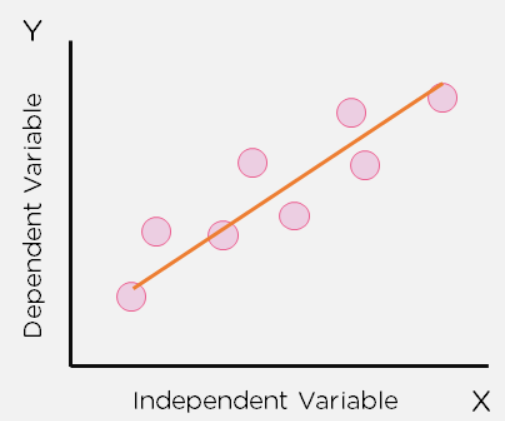
\includegraphics{screenshot001.png}
	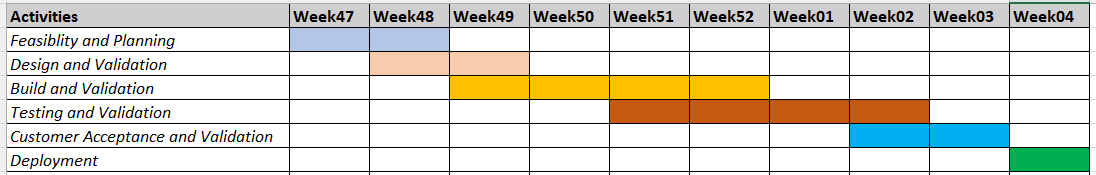
\includegraphics[width=1.2\linewidth]{images/milestone.png}
	\caption{Scheduled Milestone}
\end{figure} 

\section{Risk involved in the Project}
\label{sec:risks}
This document is a model and instructions for \LaTeX.
Please observe the conference page limits. Bla bla \newpage

\section{Data Flow Diagram}
\label{sec:data-flow}
\begin{figure}
	\centering
	%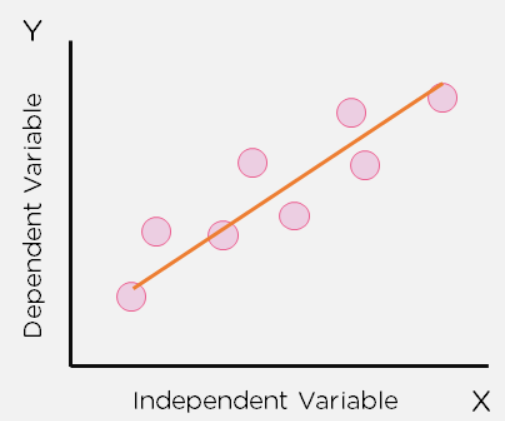
\includegraphics{screenshot001.png}
	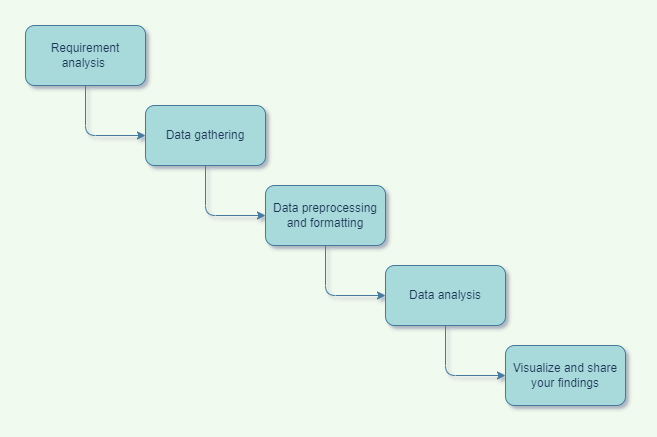
\includegraphics[width=1.2\linewidth]{images/DFD.drawio.png}
	\caption{Data Flow Diagram}
\end{figure}  \newpage

\section{Control Flow Diagram}
\label{sec:control-flow}
\begin{figure}
	\centering
	%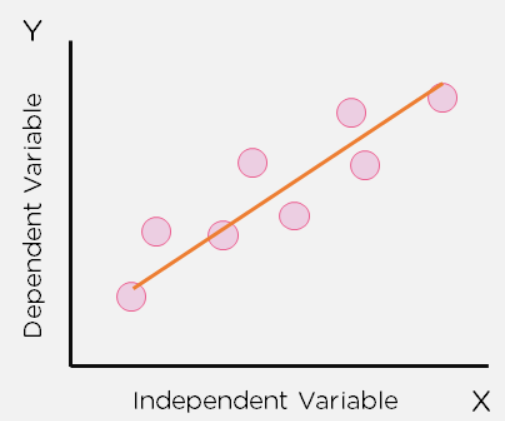
\includegraphics{screenshot001.png}
	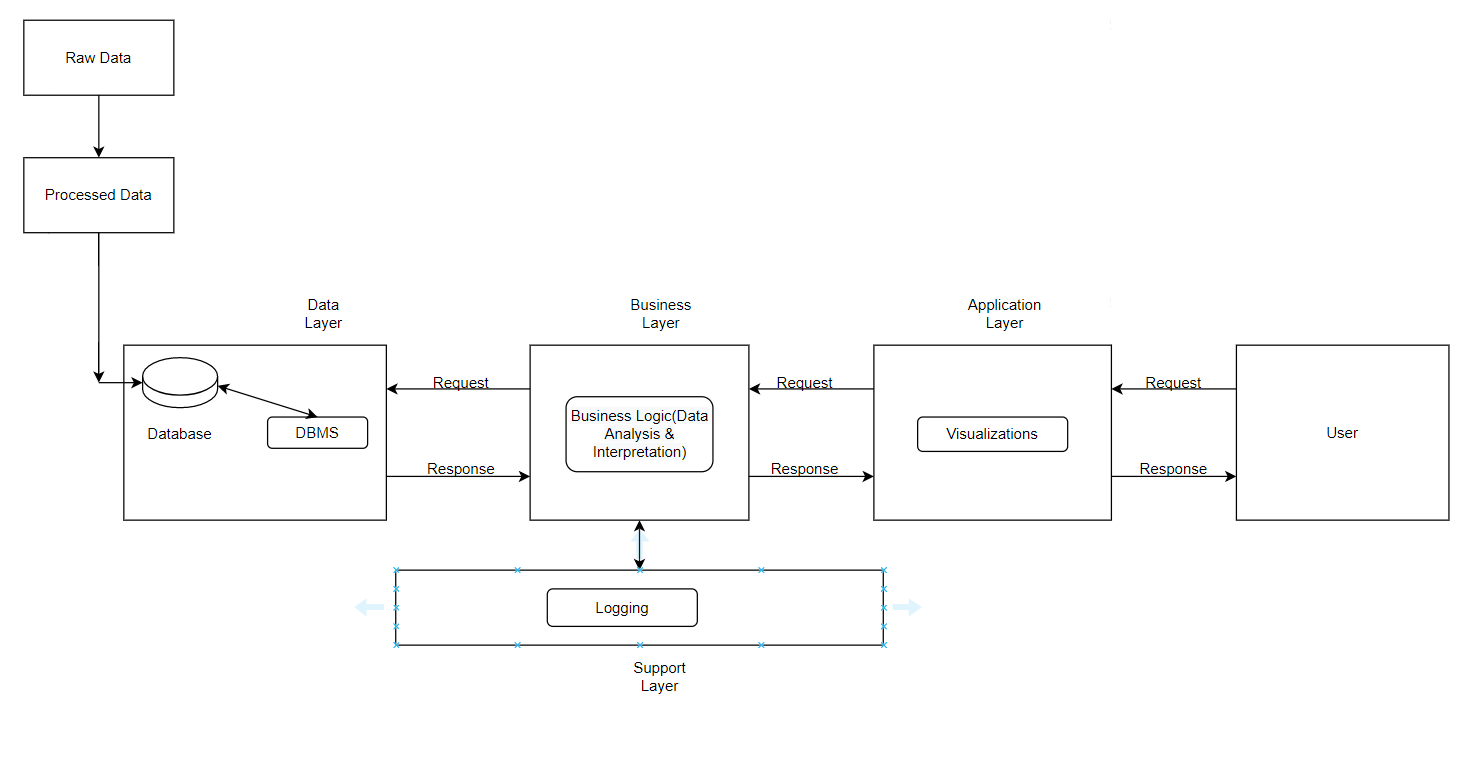
\includegraphics[width=1.2\linewidth]{images/Control Flow.png}
	\caption{Control Flow Diagram}
\end{figure} 




%%\section{Implementation of a Triple Store}

%\textbf{Here, the implementation of a triple store is described in 
%detail.}
%\textit{Here, the implementation of a triple store is described in 
%detail.}
%Here, the implementation of a triple store is described in detail.

%There are two types of implementations:
%\begin{enumerate}[a)]
%  \item Database-based implementations
% \item Other implementations
%  \item Other implementations
% \item Other implementations
%  \item Other implementations
%  \item Other implementations
%\end{enumerate}

%Apart from these two, the following have been considered in
%the literature:
%\begin{itemize}
%  \item X-based approach
%  \item Y-based approach
%  \item Z-based approach
%\end{itemize}

%\subsection{DB-based implementations}
%\lipsum[1-1]

%\subsection{Other implementations}
%\lipsum[2-2]

%%\section{Conclusion}
%\lipsum[3-3]

%\begin{thebibliography}{10}
 % \bibitem{AGVH12}
  %G. Antoniou,, P. E. Groth, F. Van Harmelen, R. Hoekstra
  %\newblock \emph{A Semantic Web Primer}.
  %\newblock The MIT Press, 2012. ISBN  978-0262018289

%\end{thebibliography}

% 	\item G. Antoniou,, P. E. Groth, F. Van Harmelen, R. Hoekstra.
% 		\emph{A Semantic Web Primer}. The MIT Press, 2012. ISBN  978-0262018289. 
% 	\item P. Hitzler, M. Kr\"otzsch, S. Rudolph, Y. Sure. 
% 		\emph{Semantic Web – Grundlagen}. Springer, 2008. ISBN 978-3-540-33993-9.
% 	\item  K. Breitman, M. A. Casanova. 
% 		\emph{Semantic Web. Concepts, Technologies and Applications (NASA 
% 		Monographs in Systems and Software Engineering)}. Springer, 2007.
% 	\item P. Szeredi, G. Lukácsy, T. Benk\"o. 
% 		\emph{The Semantic Web Explained: The Technology and Mathematics behind 
% 		Web 3.0}. Cambridge University Press, 2014. ISBN 978-0521700368.
% 	\item S. Powers. \emph{Practical RDF}. O'Reilly, 2003.
% 	\item T. Heath, C. Bizer. {\em Linked Data: Evolving the Web into a Global Data Space}. Morgan \& Claypool, 2011.
\end{document}

